\documentclass{article} % For LaTeX2e
\usepackage{iclr2018_conference,times}
\usepackage{hyperref}
\usepackage{url}
\usepackage[pdftex]{graphicx}
\usepackage{subfigure}
\usepackage{wrapfig}
\usepackage{amssymb}


%\title{Automated Aerodynamic Design using Neural Networks and Gradient Decent}
\title{Automated Design using Neural Networks and Gradient Decent}

% Authors must not appear in the submitted version. They should be hidden
% as long as the \iclrfinalcopy macro remains commented out below.
% Non-anonymous submissions will be rejected without review.

\author{Oliver Hennigh \\
Mexico\\
Guanajuato, Gto, Mexico \\
\texttt{loliverhennigh101@gmail.com} \\
}

% The \author macro works with any number of authors. There are two commands
% used to separate the names and addresses of multiple authors: \And and \AND.
%
% Using \And between authors leaves it to \LaTeX{} to determine where to break
% the lines. Using \AND forces a linebreak at that point. So, if \LaTeX{}
% puts 3 of 4 authors names on the first line, and the last on the second
% line, try using \AND instead of \And before the third author name.

\newcommand{\fix}{\marginpar{FIX}}
\newcommand{\new}{\marginpar{NEW}}

\iclrfinalcopy % Uncomment for camera-ready version, but NOT for submission.

\begin{document}


\maketitle

\begin{abstract}
In this paper, we propose a novel method that makes use of deep neural networks and gradient decent to perform automated design on complex real world problems. Our approach works by training a neural network to mimic the fitness function of the optimization task and then, using the differential nature of the neural network, we perform gradient decent to maximize the fitness. We demonstrate this methods effectiveness by designing an optimized heat sink and both 2D and 3D wing foils that maximize the lift drag ratio under steady state flow conditions. We highlight that our method has two distinct benefits. First, evaluating the neural networks prediction of fitness can be orders of magnitude faster then simulating the system of interest. Second, using gradient decent allows the design space to be searched much more efficiently.
%Automated Design is the process by which a object is designed by a computer to meet or maximize some objective. There are many examples of this such as optimizing the design of a  . Automated design is In this paper, we propose a novel method that makes use of deep neural network and gradient decent to perform automated design on complex real world problems. Our approach works by training a neural network to mimic the fittness function of the optimization task and then, using the differential nature of the neural network, we perform gradient decent to maximize the fittness. We demonstrate this methods effectiveness by designing an optimized heat sink and both 2D and 3D wingfoils that maximize the lift drag ratio under steady state flow conditions. We highlight that our method has two disticnt benifits. First, evaluating the neural networks prediction of fittness can be orders of magnatude faster then the symulating the system of interest. Second, using gradient decent allows the design space to be search much more effiently.

%Optimizing an objects geometry to have desired fluid flow properties has applications in many engineering setting such as aeornotical, automotive, and chemical engineering. In this paper, we propose a novel method that makes use of deep neural network and gradient decent to perform aerodynamic optimization of 2D and 3D airfoils in steady state flow. Our approach works by training a neural network to approximate the fluid simulation and compute values such as drag and lift. Then we use gradient decent on the parameter space of the airfoils to maximize the lift drag ratio at diffrent angles of attack. Because the network can be evaluated orders of magnatude faster then the flow solver and the gradient decent allows optimization to be performed in far fewer iterations, we are able to find optimized designs with desired properties in merr minutes vers the several days required by other flow solver based search methods. While the focus of this paper is on design of airfoils we enphasize that the methodology presented here can be used on many other automated design problems and has the potential to solve several of the key issues with automated design in general. Through out this work we present the intuition behind this.

\end{abstract}

\section{Introduction}

Automated Design is the process by which a object is designed by a computer to meet or maximize some measurable objective. This is typicaly performed by modeling the system and then exploring the space of designs to maximize some desired fittness function whether that be automotive car styling with low drag or an integrated circuit with small profile. The most notable historic example of this is the 2006 NASA ST5 spacecraft antenna designed by a evolutionary algorithm to create the best radiation pattern. More recently there has been (Flow Sculpter) and (optical computer). While there have been some significant sucesses in this feild the dream of true automated is still far from realized. The main challanges faced are heavy computational requirements for accuratly modeling the physical system under investigation and often exponentialy large search space. These two problems negatively complement eachother making the computation requirements intractable for even simple problems. For example, in the realively simple flow problems explored in this work, a heavily optimized flow solver running on modern gpus requires around 5 minutes to perform each simulation. Given that as many as 3,000 designs need to be tested to acheive reasonable performance, this results in a total computation time of 9 days on a single GPU. Increassing the resolution of the simulation or expanding the parameter space quickly make this an unrealizable problem without considerable resources.

Our approach works to solve the current problems of automated design in two ways. First, we learn a computationaly effeicent representation of the physical system on a neural network. This trained network can be used evaluate the quality or fittness of the design several orders of magnatude faster. Second, we use the differentiable nature of the trained network to get a gradient on the parameter space when performing optimization. This allows significanly more efficient optimization requiring far fewer iterations then other methods. These two abilitys of our method overcome the present difficulties with automated design and allow the previous mention 9 day optimization to be run in only 10 mins. While we only look at two relavively simple problems in this work, we enphasize that the ideas behind our method are applicable to a wide variety of automated design problems.

The first problem tackled in this work is designing a simple heat sink to maximize the cooling of a heat source. The setup of our simulation is ment to somewhat minimc the conditions seen in a heat sink on a computer processor. We keep this optimization problem realatively simple though and use this only as a first test and introduction to the method.

We also test our method on the significantly more difficult task of designing both 2D and 3D wingfoil with high lift drag ratios under steady state flow conditions. This problem is of tremendous inportance in many engineering areas such as aeornotical, aerospace and automotive engineering. Because this is a particularly challanging problem and often times unintuative for designers, there has been considerable work using automated design to produce optimized designs. We center much of the discussion in this paper around this problem because of its difficulty and view this as a true test our methods advantages and disadvantages.

As we will go into more detail in later sections, in order to perform our flow optimization tests we need a network that predicts the steady state flow from an objects geometry. This problem has previously been tackled here where they use a relatively simple network architeture. We found that better perform could be obtained using some of the modern network architecture developments. For this reason, in addition to presenting our novel method of design optimization, we also present this superiour network for predicting steady state fluid flow with nerual networks.

This work has the following contributions.
\begin{itemize}
  \item We demonstrate a novel way to use neural networks to greatly accelerate automated design.
  \item We present this method in such a way that it can ready applied to many other automated design problems.
  \item We provide a new network architeture for predicting steady state fluid flow that vastly out performs previous models.
\end{itemize}

\section{Related Work}



\section{Speeding up Computational Physics with Neural Networks}

%Predicting steady state fluid flow from object geometry was first presinted in \citep{guo2016convolutional}. In this work the authors 
Our method revoles around being able to emulate 

In recent years there has been incredable intrest in the application of neural network to computational physics problems. One of the main applications being to emulate the desired physics for less computation then the Physics simulation. Examples applications range from simulating 3D high energy particle showers seen here to 

Our method uses a network to predict steady state fluid flow from boundary conditions. This idea was first presented in \citep{guo2016convolutional} where they showed. Our flow prediction network has several key difference to this original work. First, we heavily improve the network architecture by keeping the network all convolutional and taking advantage of both residual connections and a U-Network architeture. This proved to drasticaly improve accuracy while maintain fast computation. Second, it takes in the binary representation of the boundary conditions instead of the Signed distance map. We found that with our improved network architecture, we over came the issure in their work using such a representation of the boundary.

\subsection{Automated Design Optimization of Airfoils}

To data, there has been substantial work in automated aerodynamical design for use in aeronotical and automotice applications. The standard work flow is to first parameterize the search space of designs then iteratively simulate and evaluate the. We use the A veriety of search methods have been used with some sucess in the optimization process. Simulated Annealling, Genetic Algorithms and Particle swarm have all been used with vering degrees of sucess. 


\section{Gradient Decent on Parameter Space}

\begin{figure}[h]
\begin{center}
%\framebox[4.0in]{$\;$}
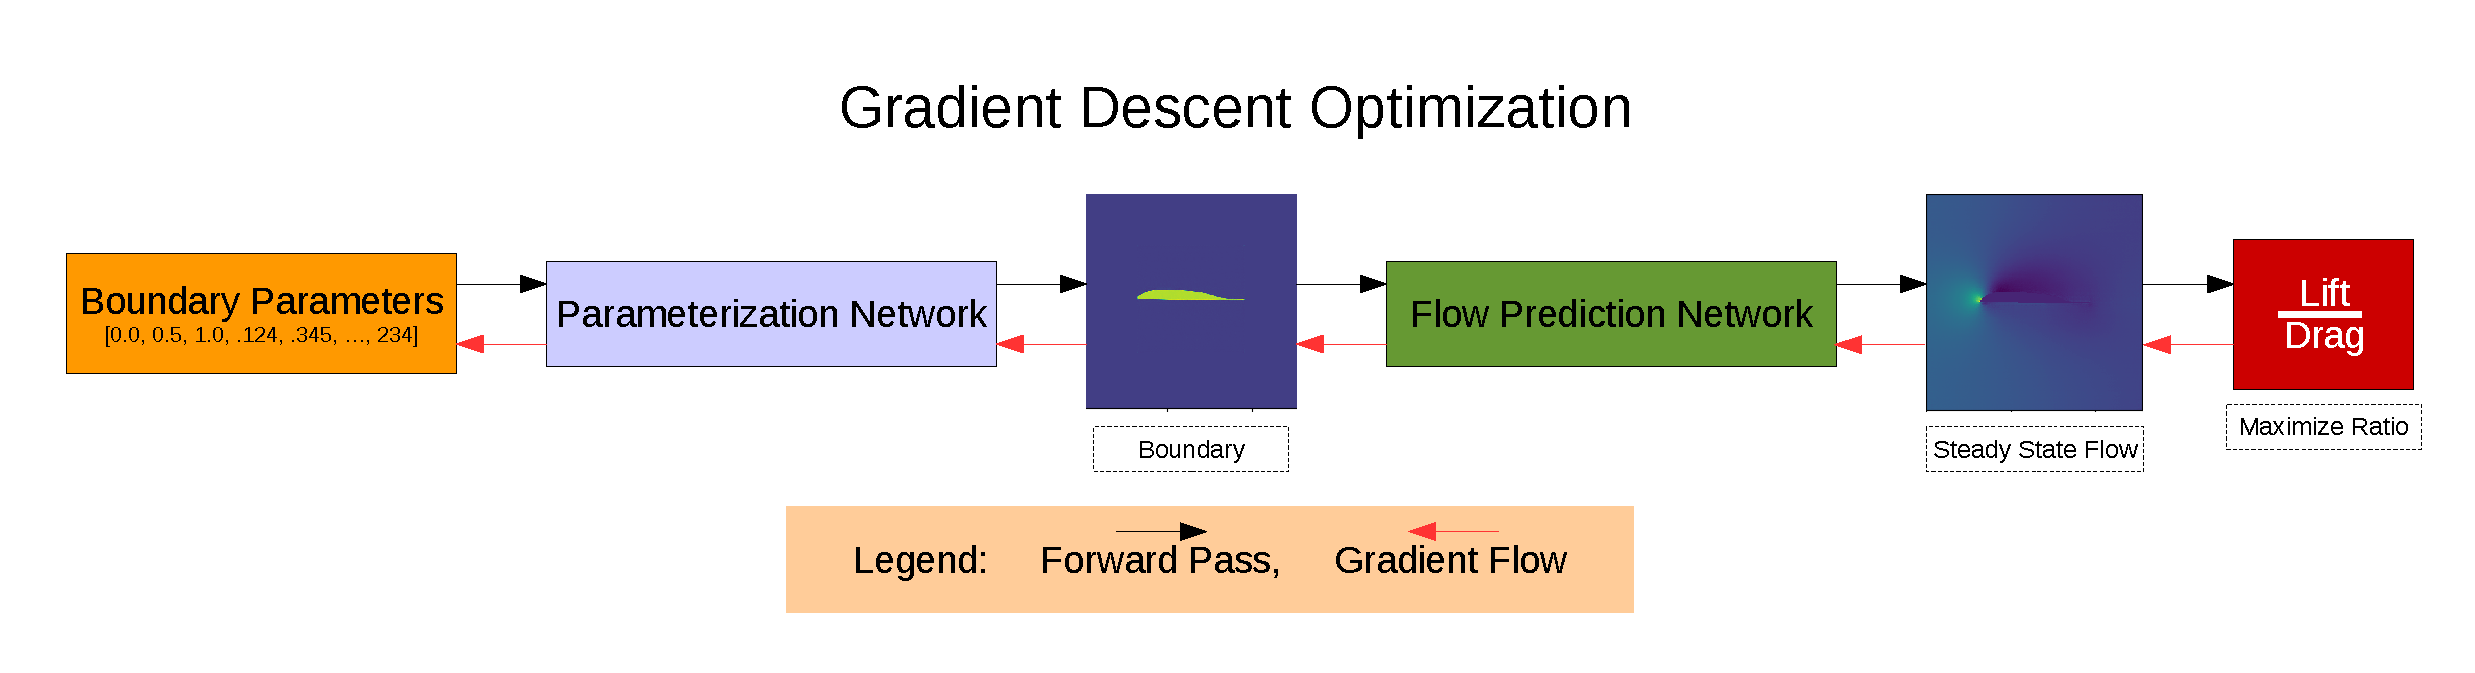
\includegraphics[scale=0.34]{./gradient_descent_optimization.pdf}
%\fbox{\rule[-.5cm]{0cm}{4cm} \rule[-.5cm]{4cm}{0cm}}
\end{center}
\caption{Illustration of Proposed Gradient Decent Method}
\end{figure}


Our automated design optimization problem can be viewed in concrete terms as maximing some desired fitness function $F(x)$ where $F:X \rightarrow \mathbb{R}$ for some space $X$ of design parameters.

\begin{equation}
  \max_{\forall x \in X} F(x)
\end{equation}

In some real world setting, evaluating the fittness function $F$ can be computationaly demanding as is the case with our fluid simulations. The first aspect of our work is to replace $F$ with a computationaly effeicent neural network $F_{net}$. This can offer considerable speed improvements as we will disscuss bellow.  The second aspect of this work is the observation that $F_{net}$ is differentiable and provided that the parameter space $X$ is real valued we can obtain a usable gradient in the direction of maximizing the fittness. This allows gradient decent to be performs where as in most setting $F$ is not differentable and requires other search techniques such as simulated annealing or genetic algorithms. This allows faster optimization to be performed with fewer iterations as we will demonstrate bellow. The requirement of $X$ to be real valued presents some chalanges though. To show case this and our solutions to them we go through the example problem of optimizing the fin height on a heat sink.

In our simple heat sink problem, $X$ contains 15 real valued parameters between 0 and 1. Each of these parameters corrisponds to the height of an aluminum fin on the heat sink as seen in the figure. In our optimization problem we assume that there is a fixed amount of aluminum and scale the total lenghth of all the fins to meet this requirement. The presents an intereseting problem of deteremining the optimal length each fin should have to maximize the cooling of the heat source. The simplest application of our method would be to have a neural network to take in the 15 fin height values and output a single value corresponding to the tempuature at the heat source. This apporach has the draw back that if you want to add another aspect to the optimization like makeing sure the left side is cooler then the right side you would need to retrain the network. Another solution is to have the network again take in the fin parameters but output the full heat distrobution of heat sink. This allows diffrent quantitize to be optimized but is still limiting in that our network only runs on a single parameter set up. Our solution to this problem is to train two networks. The first network, $P^{heat}_{net}$, takes in the fin parameters and generates a binary image corresponding to the geometry of the heat sink. We refer to this as the parameterization network. The second network, $S^{heat}_{net}$, predicts the steady state heat distorbution from the geometry. Because the parameterization network is performing an extremely simple task and training data can be generating cheaply, we can quickly retrain $P^{heat}_{net}$ if we want to change the parameter space. The same approach is used for the steaty state flow problem and a figure dipicting this can be found here. This approach allows our network to be as veratile as possible while still allowing it to used on many design optimization tasks.

Up until now we have not discussed how to generate data needed to train these neural neural networks. Generateing the data to train the parameterization network is realitively simple. If the paraeterization we are using is known we simply make a set of parameter vectors and there corissponding geometrys. In the case of the heat sink this is a set of examples composed of the 15 parameters and there corrisponding binary representation of the head sink. Putting together a dataset for $S^{heat}_{net}$ or $S^{flow}_{net}$ (fluid flow network) is somewhat more complicated though. The simplest solution and the apporoch used in this work is to simulate the respective physics on objects drawn from the object design space. For the heat sink problem this would entail a dataset of object geometrys and their corrisponding steady state heat distrobutions. This method has the disadvantage that the network only sees examples from the current parameter search space and if it is changed the network may not be able to accuratly predict the physics. We argue this is not a significate issue for several reasons. First, in the work seen here the network is able to generalize effectively to objects outside its train set. During the course of this work we tested our network on a veriety of datasets and found similar generaling abilities. Second, it is easy imagine a setup where a network is trained on a large set of diverse simulations and then finetuned on the current desired parameter space when desired. For these reasons we feel that this approach of generating simulation data is not significantly limiting and feel that employing some highbread approach would only distract from the underlying method presented.

\subsection{Flow Prediction Network}

The core componet of our method is being able to emulate the physics simulation with a neural network. For the steady state flow problem here has already been work doing just this found here. As mentioned above, we have made some improvements to this network architecture design. A figure illustrating our network can be found here. This model resembols the u-network architeture seen here with a series skip after each down sample. The advantages of this style of network are its high performance on image to image type tasks, trainablility on small datasets, and fast evaluation time in comparison to networks with large fully connected layers. The trainability on small datasets make this particulary effective on predicting steady state flow because generating simulation data to train on is time consuming. Our network is able to train on realively small datasets of only 4,000 flow simulation in comparision to the 100,000 required in previous work predicting steady state flow. Other modifications we have used are the use of gated residual blocks blocks that allow the gradient to be propogated extremely effeicently and heavely lowers training time.

\section{Experiments}

%In the following sections we subject our method and model to a variety of test in order to see its performance. Because our method is centered around gradients oThe goal being first to determine how accuraty and fast our model can predict steady state flow. In particular, what its accuracy in predicting values such a drag and lift as these are important quantitize in our optimization. Second, we investigate how effective our gradient decent optimization is. This line of tests compares our method to other none gradient based search techniques and illustrates what is happening in the optimization processes looks like. For example, what does the gradient surface look like.

\subsection{Datasets}

To train the parameterization networks we generated a set of 10,000 examples for each system consisting of a parameter vector and their corrisponding geometry. 

The heat sink simulations dataset consists of BLANK training examples simulated with implicit finite difference method.

\subsection{Training}

For all networks we used the adam optimizer. For $S^{heat}_{net}$ or $S^{flow}_{net}$ a learning rate of 0.0001 was used until the loss platued and then the learning rate was dropped to 0.00001. Mean Squared Error was used as the loss function however for the flow prediction network we scaled up the loss from the pressure field by 30 to roughly match the loss from the velocity vector field. Without this modification the network would train much slower and only learn the pressure field once the velocity vector field was firmly learned. During the course of this work other loss functions were experimented with such as adding a loss term in predicting the fluid flow forces on the object. This had benificial effects but complicated the method and is specific to fluid flow so was left out from the final network. The parameterization networks also used Mean Squared Error with a constant learning rate of 0.0001. We found the parameterization networks trained extremely quickly and reqiured little parameter optimization.

\subsection{Gradient Decent Design Optimization Details}

There are some complexities in how exactly to the design parameters are optimizaed that need explination. When training the parameterization network, the raw design parameters are used from there respective ranges and sent through the network. During design optimization however, the trainable design parameters go through a hard sigmoid functions and then are scaled to there apropriote range before being sent through the parameterization network. This presents a challage because if the parameters leave the range -1 and 1 the gradient will go to zero and they will be stuck at that value for the diration of the optimization. We overcame this problem by placeing a small loss on any parameter greator 1 or less then -1. This prevents the parameters from getting stuck and allows mobiliy for the entire optimization process.

One expected difficulty in optimizing the parameters is falling into local optima. We apply momentum and add a wee bit noise to the params

\subsection{Heat Sink Optimization}

As discussed above, the heat sink optimization task is to find a set of fin heights that maximaly cool a constant heat source given a fixed total lenght of the fins. The set up roughly corrisponds to an aluminum heat sink placed placed on a cpu where the heat source is treated as addition of tempurature. There is no heat disipation between the underside of the heat sink but all other areas not on the heat sink are kept at a constant tempurature. The heat diffusion constant in the heat sink is kept at 1000 and the diffusion constant at the boundarys is 10. The intuative solution to this optimization problem is to place long fins near the heat source and shorter fins farther away. Balancing this is a difficult task though because changing the length of any fin has a global effect on how much heat is disipaed by all the other fins. 

After training our networks $P^{heat}_{net}$ and $S^{heat}_{net}$ we perform our proposed gradient optimization on the 15 fin heights to minizize the tempurature at the source. In figure \ref{heat_sink_optimization} we see the optimized heat sink and see that the design resebles what our intuition tells us. We also not the extremely smooth optimization that occurs with only small bumps caused by the small addition of noise.

\begin{figure}[!t]
\begin{center}
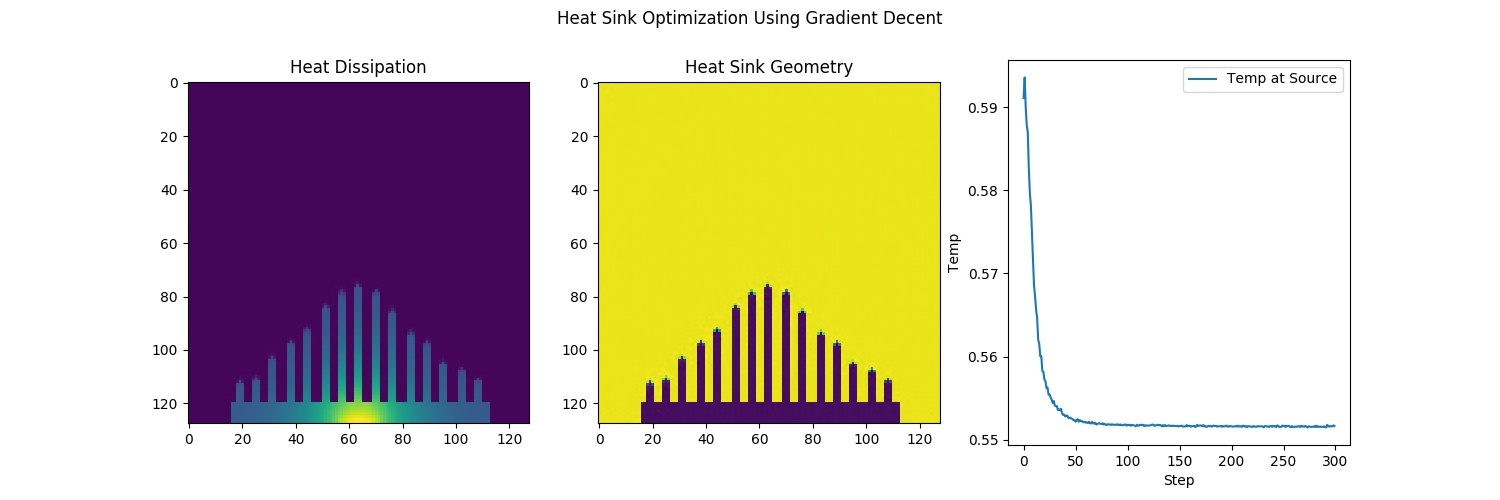
\includegraphics[scale=0.30]{../test/figs/heat_learn_gradient_decent.jpeg}
\end{center}
\caption{Optimization of heat sink using our gradient decent method.}
\label{heat_sink_optimization}
\end{figure}

In order to get a s

\begin{figure}[h]
\begin{center}
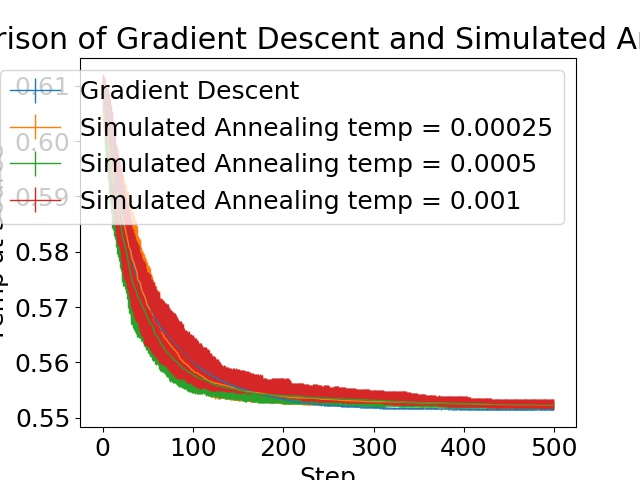
\includegraphics[scale=0.30]{../test/figs/heat_learn_comparison.jpeg}
\end{center}
\caption{A comparison of our gradient decent based method and simulated annealing in optimizing the design of a heat sink. Several starting tempurature for the simulated annealing algorithm are provided. Each optimization was performed 40 times from the same starting design and the bars show the standard deviation over these runs.}
\end{figure}


\subsection{Flow Prediction Accuracy}



\begin{figure}[!t]
\begin{center}
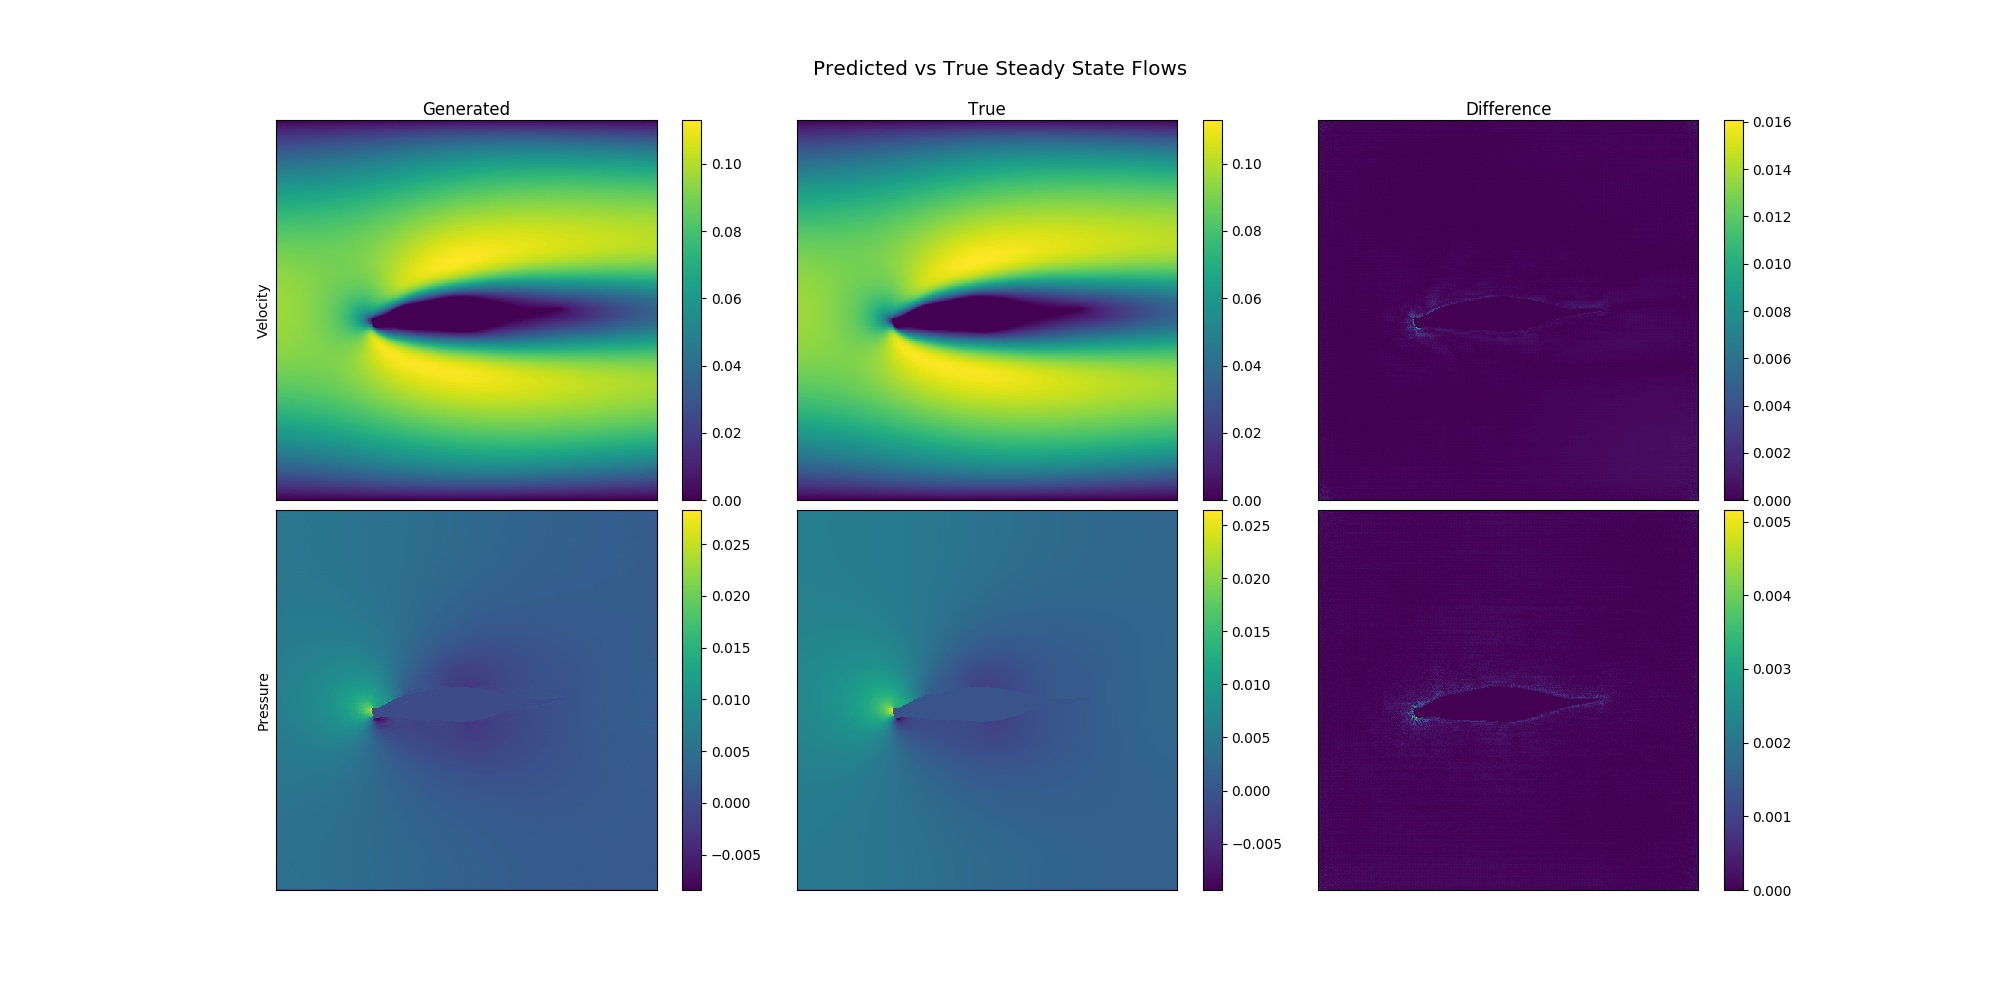
\includegraphics[scale=0.30]{../test/figs/generated_flow_difference.jpeg}
\end{center}
\caption{Comparison of steady state flow predicted by neural network and the lattice boltzmann flow solver.}
\label{flow_accuracy}
\end{figure}

\begin{figure}[h]
\begin{center}
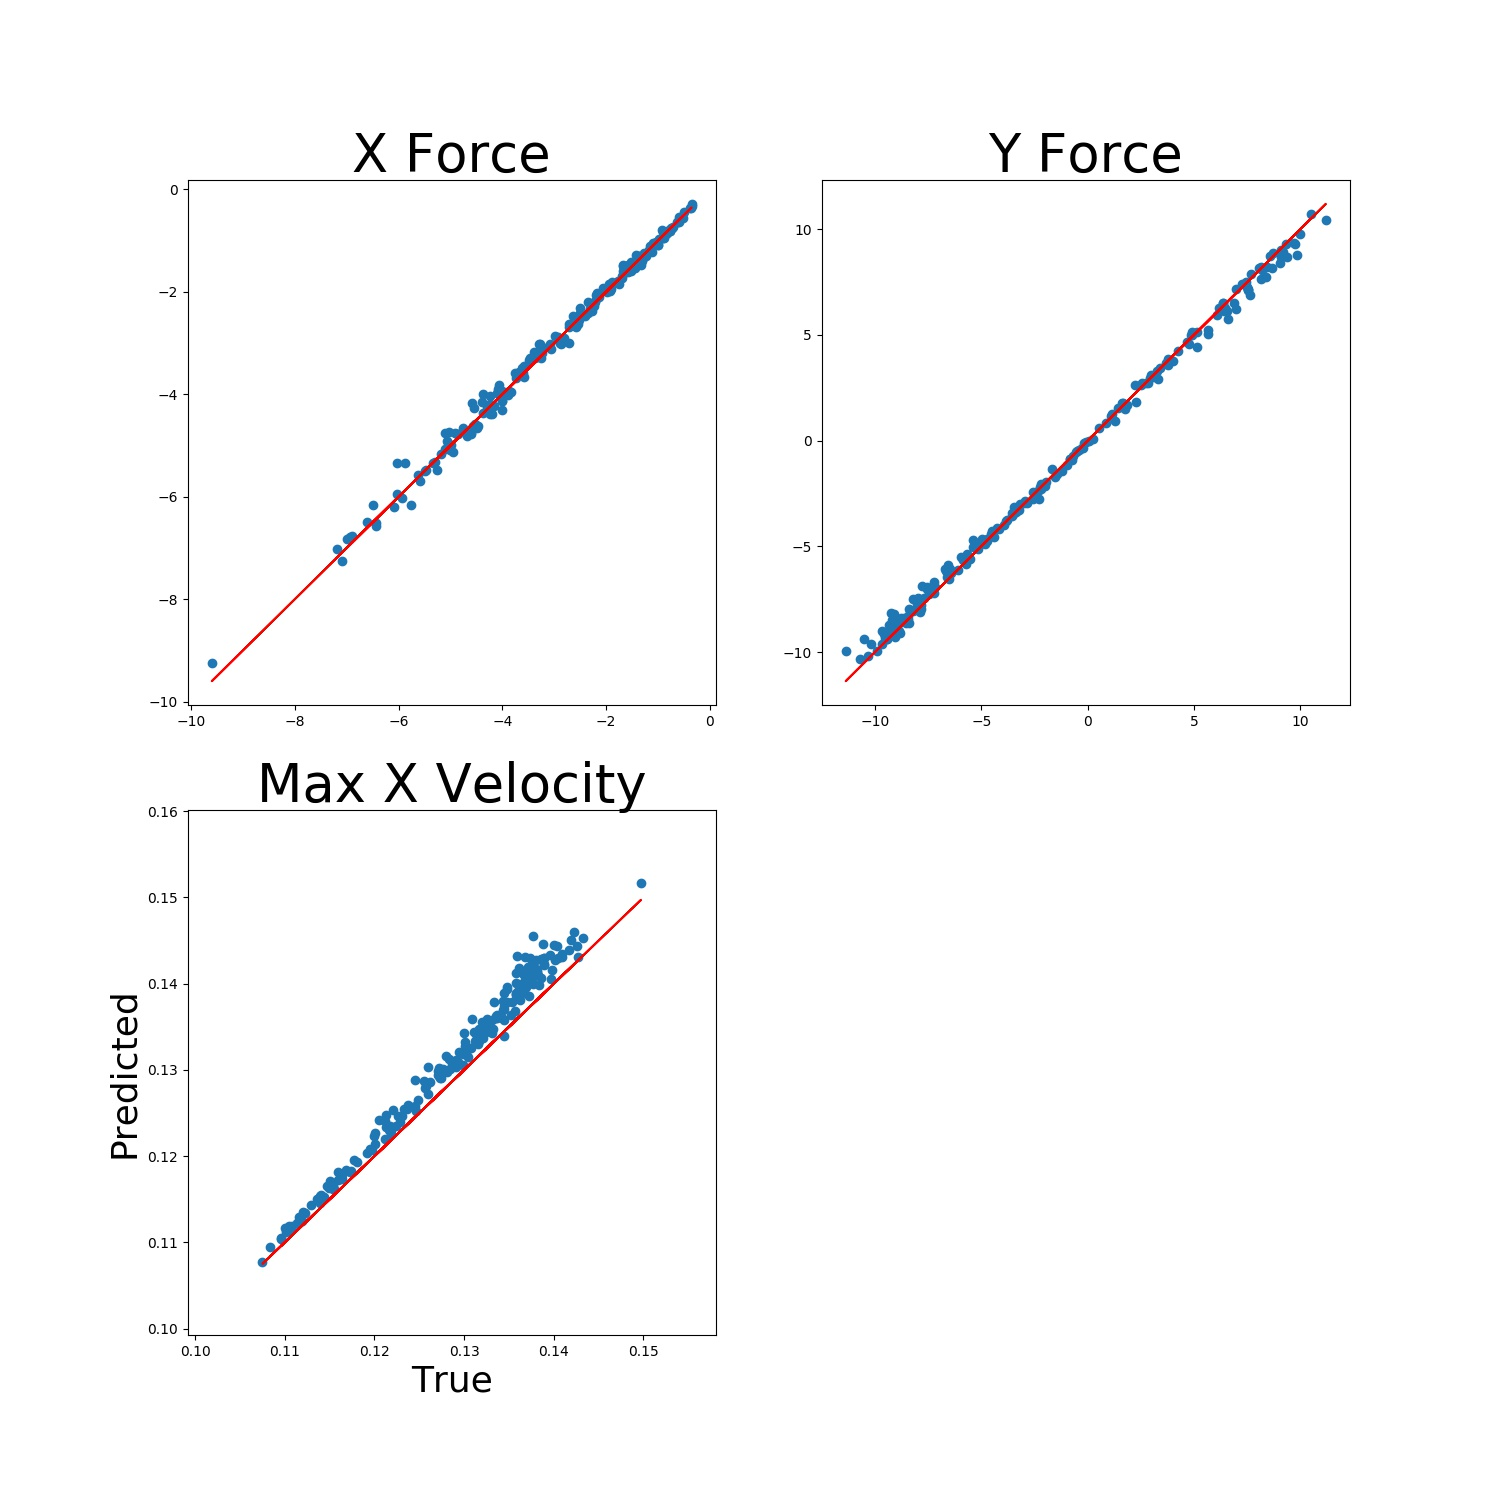
\includegraphics[scale=0.30]{../test/figs/flow_accuracy_2d.jpeg}
\end{center}
\caption{Accuracy of the neural network in predicted various quantities.}
\end{figure}

\subsection{Automated Design of 2D and 3D Airfoils}

\begin{figure}[h]
\begin{center}
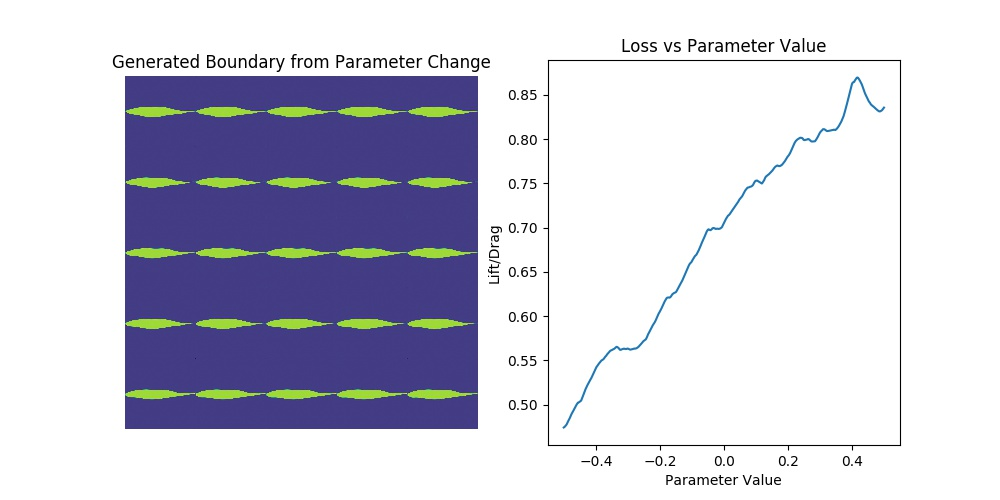
\includegraphics[scale=0.30]{../test/figs/boundary_space_explore.jpeg}
\end{center}
\caption{A look at the design }
\end{figure}

\begin{figure}[h]
\begin{center}
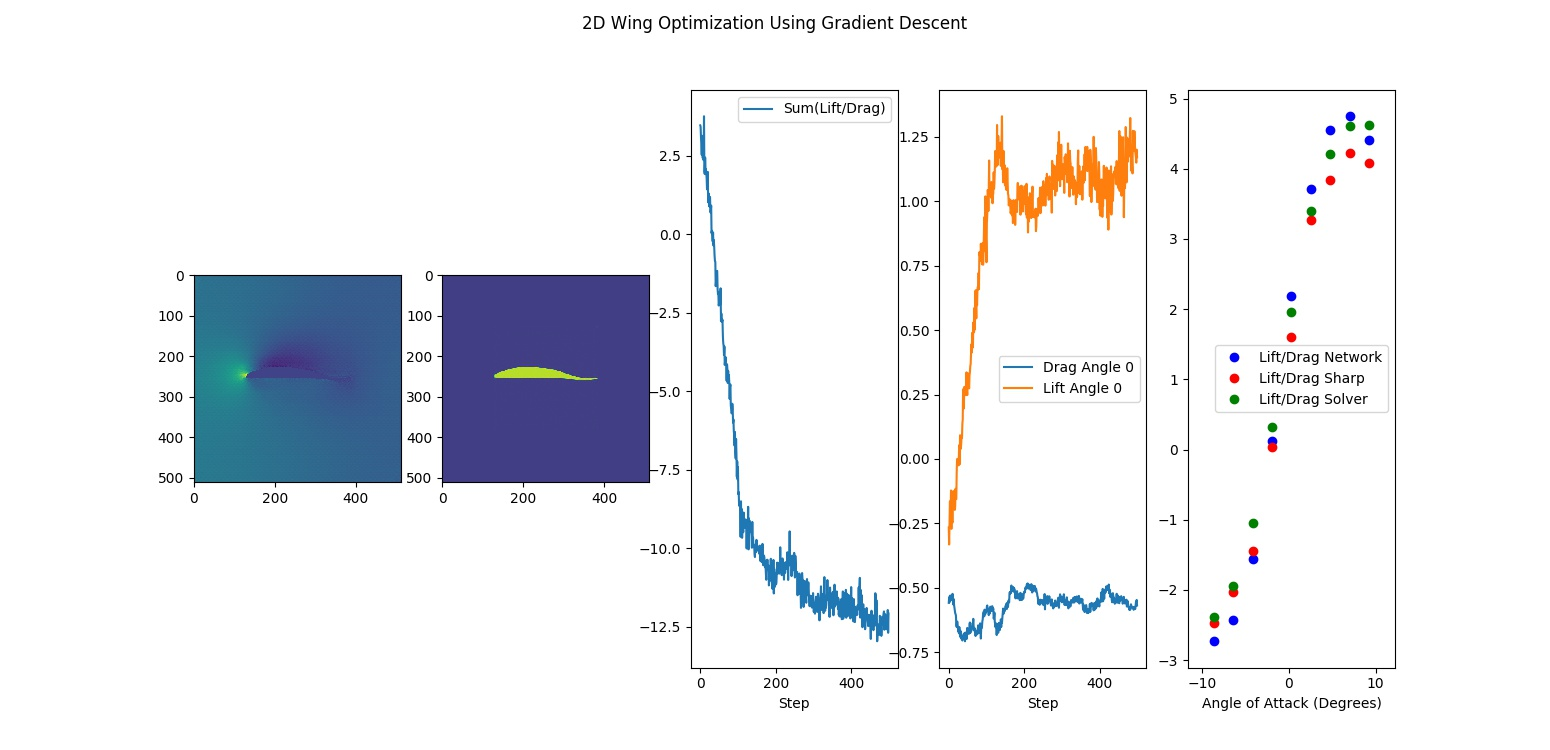
\includegraphics[scale=0.30]{../test/figs/learn_gradient_descent.jpeg}
\end{center}
\caption{Flow}
\end{figure}

\begin{figure}[h]
\begin{center}
\includegraphics[scale=0.30]{../test/figs/learn_comparsion.jpeg}
\end{center}
\caption{Flow}
\end{figure}

\subsection{Comparison of Computation Times}



\section{Conclusion}

In this work we hav


\section{Sample Tables}

\begin{table}[t]
\caption{Sample table title}
\label{sample-table}
\begin{center}
\begin{tabular}{l|lllll}
Batch Size & 1 & 2 & 4 & 8 & 16 \\ \hline 
Flow Net $512^2$ & 0.150 sec & 0.101 sec & 0.077 sec & 0.065 sec & 0.058 sec \\ 
Param Net $512^2$ & 0.083 sec & 0.045 sec & 0.026 sec & 0.015 sec & 0.011 sec \\ 
Learn Step $512^2$ & 0.494 sec & 0.345 sec & 0.270 sec & 0.231 sec & Nan \\ 
Flow Net $144^3$ & 0.826 sec & 0.686 sec & 0.627 sec & 0.623 sec & Nan \\ 
Param Net $144^3$ & 0.195 sec & 0.144 sec & 0.119 sec & 0.106 sec & 0.093 sec \\ 
Learn Step $144^3$ & 3.781 sec & Nan & Nan & Nan & Nan \\ 
\end{tabular}
\end{center}
\end{table}


\subsubsection*{Acknowledgments}

This work was made possible through the \url{http://aigrant.org} run by Nat Friedman and Daniel Gross. This work would not have be possible without this very genourous support.

\bibliography{iclr2018_conference}
\bibliographystyle{iclr2018_conference}

\section{Appendix}

\begin{figure}[h]
\begin{center}
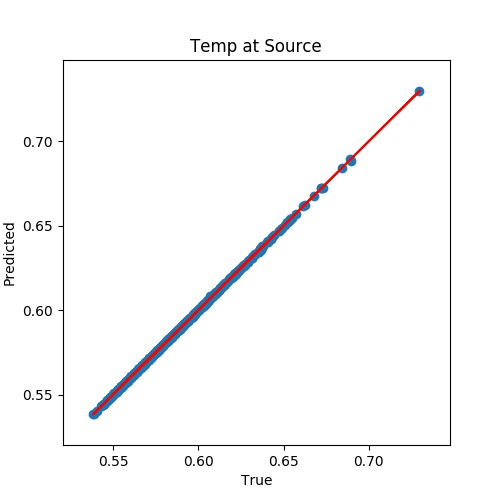
\includegraphics[scale=0.15]{../test/figs/heat_accuracy.jpeg}
\end{center}
\caption{Flow}
\end{figure}


\begin{figure}[h]
\begin{center}
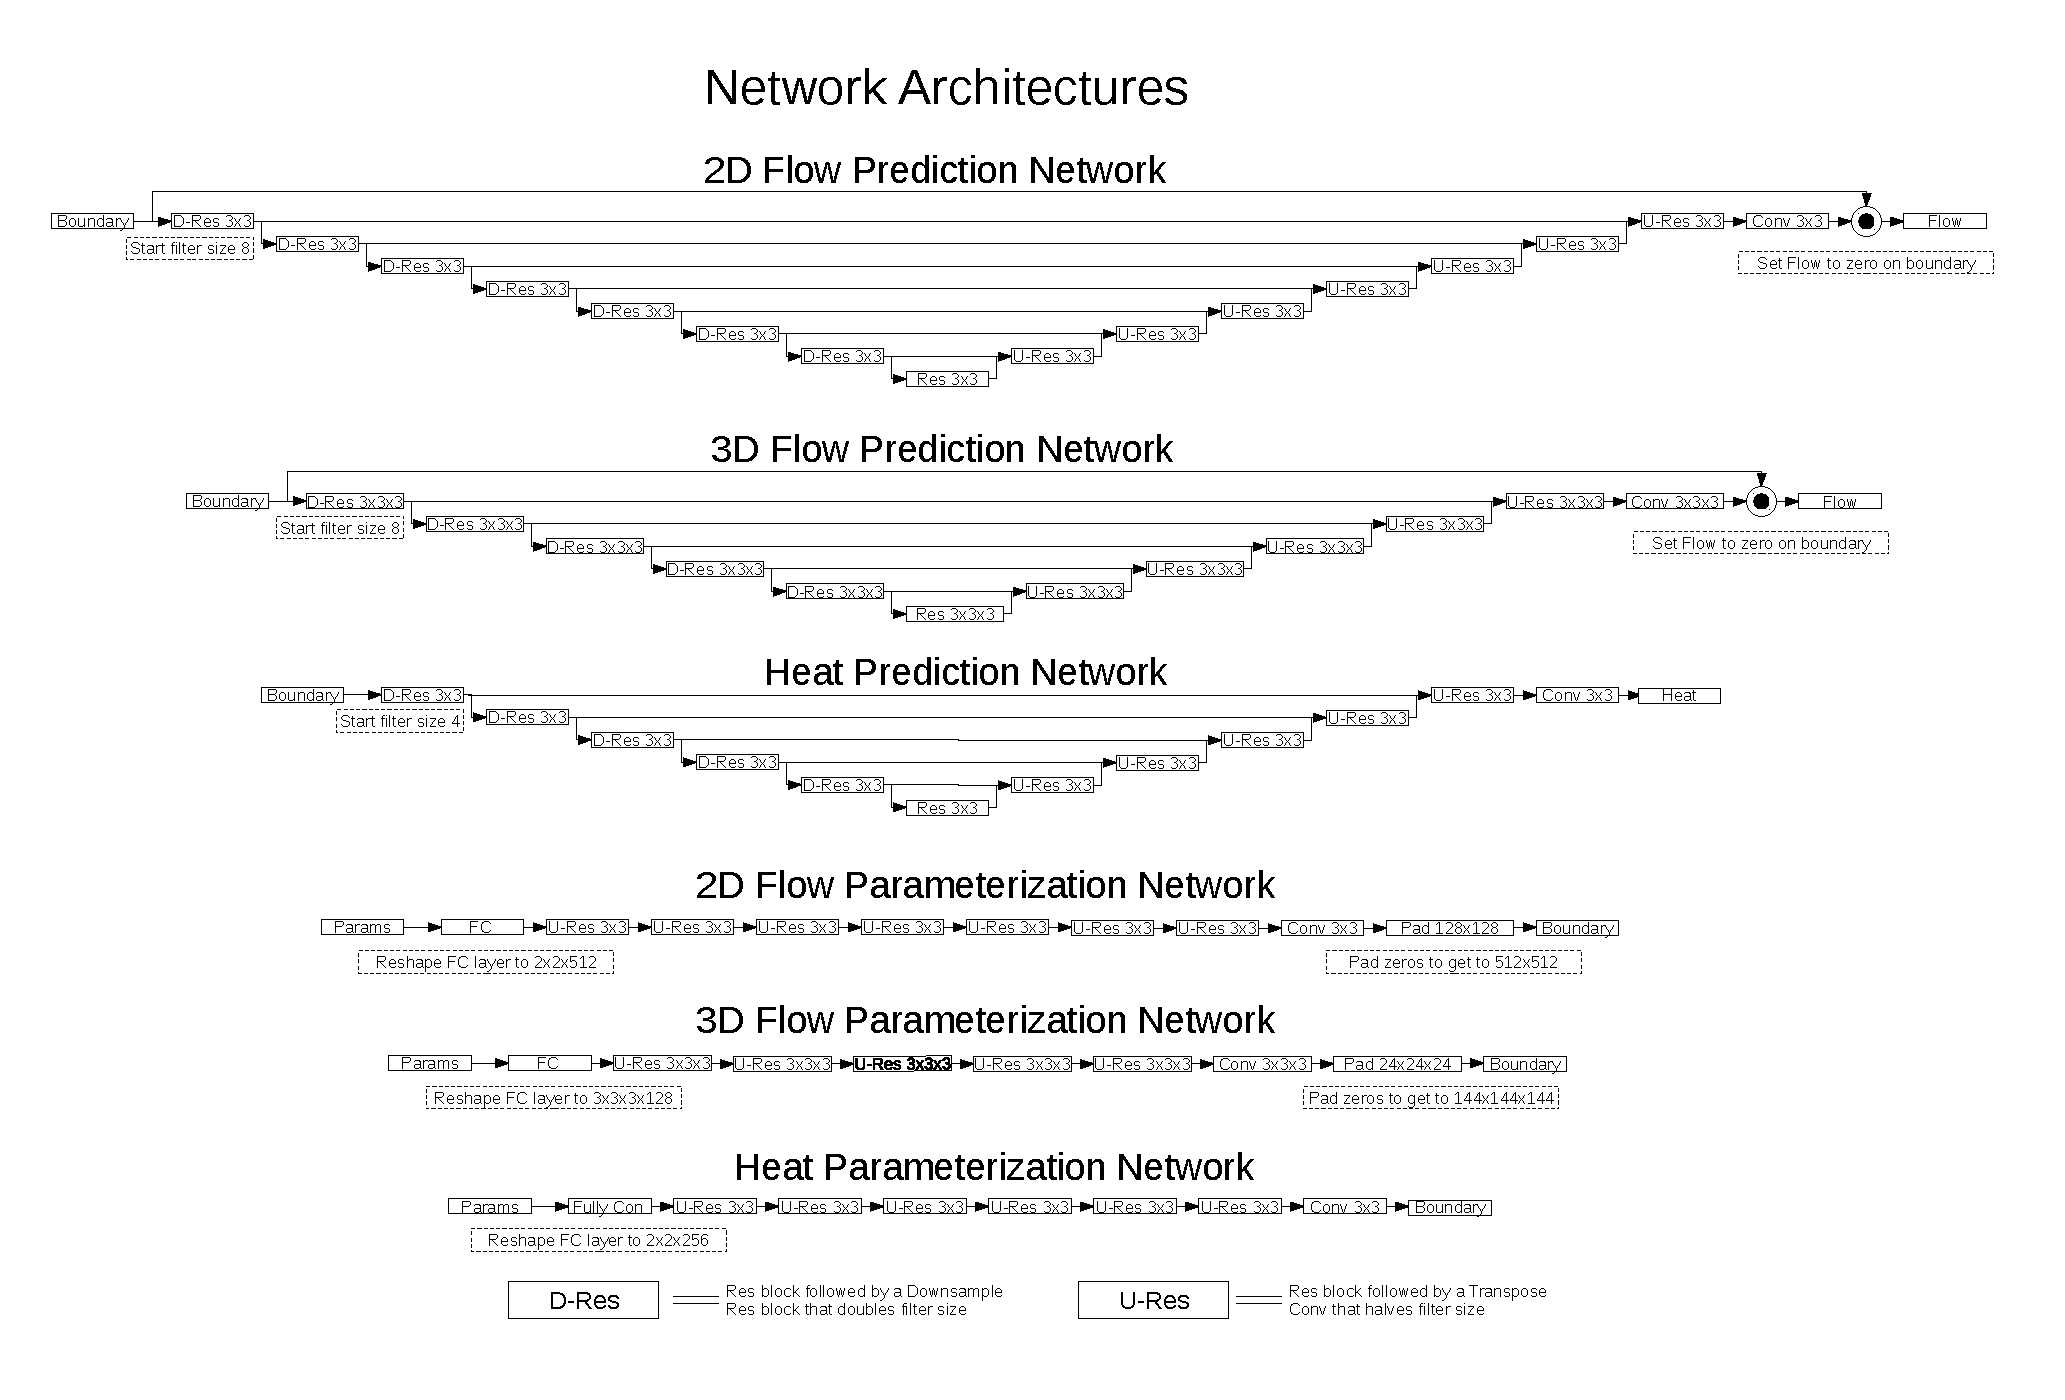
\includegraphics[scale=0.45]{./appendix_flow_net.pdf}
\end{center}
\caption{Flow}
\end{figure}

\end{document}
